\section{Deskriptive Statistik}\label{sec:deskriptive-statistik}

\begin{terms}{Begriffe}
    \\
    \begin{itemize}
        \item \textbf{Merkmalsträger / Statistische Einheiten}: Objekte, an denen interessierende Größen erfasst werden (z. B. Menschen, Unternehmen).
        \item \textbf{Grundgesamtheit}: Alle statistischen Einheiten, über die Aussagen getroffen werden sollen (z. B. alle Mietwohnungen in Zürich).
        \item \textbf{Vollerhebung}: Datenerhebung bei jeder Einheit der Grundgesamtheit. Oft nicht nötig oder zu aufwendig.
        \item \textbf{Stichprobe}: Teilmenge der Grundgesamtheit, die möglichst repräsentativ sein soll. Meist eine Zufallsstichprobe.
        \item \textbf{Stichprobengröße}: Anzahl der Einheiten in der Stichprobe.
        \item \textbf{Merkmal (Variable)}: Interessierende Größe, die an den Merkmalsträgern gemessen wird (z. B. Nettomiete, Baualter).
        \item \textbf{Ausprägungen}: Mögliche Werte, die ein Merkmal annehmen kann (z. B. Geschlecht: männlich, weiblich, divers).
    \end{itemize}
\end{terms}

\tikzset{every node/.style={font=\fontsize{8}{9}\selectfont}}

\begin{tikzpicture}
    [
    node distance=0.2cm and 1.0cm,
    box/.style={draw, rounded corners, text centered, text width=0.25\columnwidth, minimum height=1.2cm, inner sep=3pt},
    title/.style={font=\bfseries\fontsize{8}{9}\selectfont, minimum height=0.5cm},
    arrow/.style={->, thick}
    ]

    % Main title box
    \node (main) [box, title] {Merkmalstyp};

    % Top row (Qualitativ and Quantitativ)
    \node (qualitativ) [box, below left=of main, xshift=2cm, yshift=-0.3cm, text width=0.4\columnwidth, minimum height=1.6cm] {\textbf{Qualitativ/Kategoriell}\\\textcolor{darkblue}{Es wird eine Ausprägung, aber kein Ausmaß angegeben. Nur endlich viele Ausprägungen.}};
    \node (quantitativ) [box, below right=of main, xshift=-2cm, yshift=-0.3cm, text width=0.4\columnwidth, minimum height=1.6cm] {\textbf{Quantitativ/Metrisch}\\\textcolor{darkblue}{Es wird ein Ausmaß in Zahlen angegeben.}};

    % Bottom row for Qualitativ (Nominal and Ordinal)
    \node (nominal) [box, below=of qualitativ, xshift=-1.21cm, yshift=-0.3cm, text width=0.215\columnwidth] {\textbf{Nominal}\\\textcolor{darkblue}{Keine Ordnung, reine Kategorisierung.}};
    \node (ordinal) [box, below=of qualitativ, xshift=1.21cm, yshift=-0.3cm, text width=0.215\columnwidth] {\textbf{Ordinal}\\\textcolor{darkblue}{Ordnung vorhanden, Rangierung möglich.}};

    % Bottom row for Quantitativ (Diskret and Stetig)
    \node (diskret) [box, below=of quantitativ, xshift=-1.21cm, yshift=-0.3cm, text width=0.215\columnwidth] {\textbf{Diskret}\\\textcolor{darkblue}{Endliche oder abzählbar unendlich viele Ausprägungen.}};
    \node (stetig) [box, below=of quantitativ, xshift=1.21cm, yshift=-0.3cm, text width=0.215\columnwidth] {\textbf{Stetig}\\\textcolor{darkblue}{Alle Werte in einem reellen Intervall.}};

    %%% Arrows from Main to Qualitativ and Quantitativ %%%
    % Vertical line from the main node down to the split point (no arrow)
    \draw (main.south) -- ++(0,-0.2) coordinate(midSplit);

    % Horizontal lines (no arrow) from the split point to the child nodes
    \draw (midSplit) -- (qualitativ.north |- midSplit);
    \draw (midSplit) -- (quantitativ.north |- midSplit);

    % Final vertical arrows to the child nodes
    \draw [->] (qualitativ.north |- midSplit) -- (qualitativ.north);
    \draw [->] (quantitativ.north |- midSplit) -- (quantitativ.north);

    %%% Arrows from Qualitativ to Nominal and Ordinal %%%
    % Vertical line from Qualitativ down to the split point (no arrow)
    \draw (qualitativ.south) -- ++(0,-0.2) coordinate(splitQualitativ);

    % Horizontal lines (no arrow) from the split point to Nominal and Ordinal
    \draw (splitQualitativ) -- (nominal.north |- splitQualitativ);
    \draw (splitQualitativ) -- (ordinal.north |- splitQualitativ);

    % Final vertical arrows to the child nodes
    \draw [->] (nominal.north |- splitQualitativ) -- (nominal.north);
    \draw [->] (ordinal.north |- splitQualitativ) -- (ordinal.north);

    %%% Arrows from Quantitativ to Diskret and Stetig %%%
    % Vertical line from Quantitativ down to the split point (no arrow)
    \draw (quantitativ.south) -- ++(0,-0.2) coordinate(splitQuantitativ);

    % Horizontal lines (no arrow) from the split point to Diskret and Stetig
    \draw (splitQuantitativ) -- (diskret.north |- splitQuantitativ);
    \draw (splitQuantitativ) -- (stetig.north |- splitQuantitativ);

    % Final vertical arrows to the child nodes
    \draw [->] (diskret.north |- splitQuantitativ) -- (diskret.north);
    \draw [->] (stetig.north |- splitQuantitativ) -- (stetig.north);

\end{tikzpicture}

\begin{remark}
    \textbf{Häufigkeiten und Verteilungsfunktion}
\end{remark}

\renewcommand{\arraystretch}{1.2}

\begin{concept} {\textbf{NICHT klassiert:}}
    \\\\
    \begin{tabular}{|p{5cm}|c|c|c|c|c|c|}
        \hline
        $a_i$                                              & 5              & 6              & 7              & 8              & 9              \\
        \hline
        \multirow{1}{*}{absolute Häufigkeit $n_i$}         & 1              & 3              & 4              & 1              & 1              \\
        \hline
        \multirow{1}{*}{relative Häufigkeit $f_i$}         & $\frac{1}{10}$ & $\frac{3}{10}$ & $\frac{2}{5}$  & $\frac{1}{10}$ & $\frac{1}{10}$ \\
        \hline
        \multirow{1}{*}{kummulative rel. Häufigkeit $F_i$} & $\frac{1}{10}$ & $\frac{4}{10}$ & $\frac{8}{10}$ & $\frac{9}{10}$ & 1              \\
        \hline
    \end{tabular}
    \\
    \begin{itemize}
        \item \textbf{absolute Häufigkeit $n_i$}: Anzahl der Beobachtungen, die den Wert $a_i$ annehmen.
        \item \textbf{relative Häufigkeit $f_i$}: Anteil der Beobachtungen, die den Wert $a_i$ annehmen.
        \item \textbf{kummulative relative Häufigkeit $F_i$}: Anteil der Beobachtungen, die den Wert $a_i$ oder kleiner annehmen.
    \end{itemize}

    \pgfplotsset{compat=1.17} % Ensures compatibility

    % Probability Mass Function (PMF)
    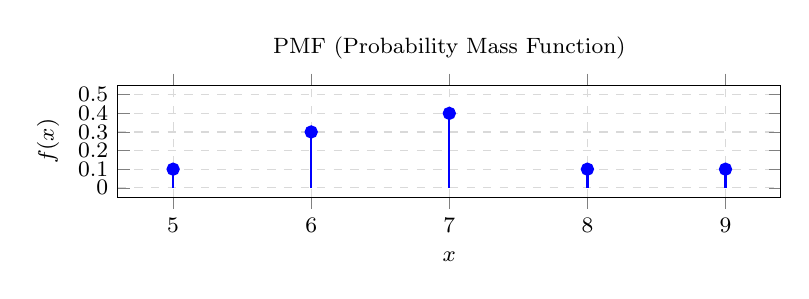
\begin{tikzpicture}
        \begin{axis}
            [
            ybar, % Bar plot
            ymin=0, ymax=0.5,
            enlargelimits=0.1,
            ylabel={$f(x)$},
            xlabel={$x$},
            xtick={5,6,7,8,9},
            ytick={0, 0.1, 0.2, 0.3, 0.4, 0.5},
            title={PMF (Probability Mass Function)},
            grid=major,
            grid style={dashed, gray!30},
            width=10cm,
            height=3cm
            ]
            \addplot+[
            ycomb,
            blue,
            thick,
            mark=*,
            mark options={solid, fill=blue}
            ] coordinates {
                (5, 0.1)
                (6, 0.3)
                (7, 0.4)
                (8, 0.1)
                (9, 0.1)
            };
        \end{axis}
    \end{tikzpicture}

% Cumulative Distribution Function (CDF)
    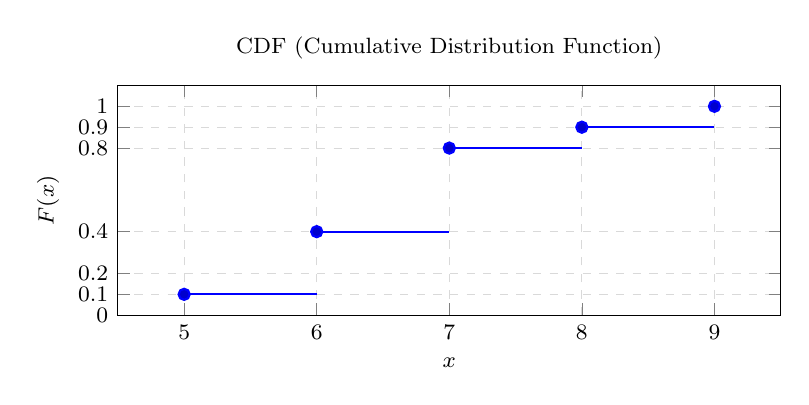
\begin{tikzpicture}
        \begin{axis}
            [
            ymin=0, ymax=1.1,
            xmin=4.5, xmax=9.5,
            ylabel={$F(x)$},
            xlabel={$x$},
            xtick={5,6,7,8,9},
            ytick={0, 0.1, 0.2, 0.4, 0.8, 0.9, 1},
            title={CDF (Cumulative Distribution Function)},
            grid=major,
            grid style={dashed, gray!30},
            width=10cm,
            height=4.5cm
            ]
            \addplot+[
            const plot,
            jump mark left,
            blue,
            thick
            ] coordinates {
                (5, 0.1)
                (6, 0.4)
                (7, 0.8)
                (8, 0.9)
                (9, 1.0)
            };
        \end{axis}
    \end{tikzpicture}
\end{concept}

\begin{concept} {\textbf{Klassiert:}}
    \\\\
    \begin{tabular}{|c|c|c|c|}
        \hline
        % First row with intervals
        & $[4, 6)$       & $[6, 8)$       & $[8, 10)$      \\
        \hline
        % Second row: n_i
        $n_i$                 & 1              & 7              & 2              \\
        \hline
        % Third row: f_i
        $f_i$                 & $\frac{1}{10}$ & $\frac{7}{10}$ & $\frac{2}{10}$ \\
        \hline
        % Fourth row: Klassengröße d_i
        Klassengröße $d_i$    & 2              & 2              & 2              \\
        \hline
        % Fifth row: PDF
        PDF $\frac{f_i}{d_i}$ & $\frac{1}{20}$ & $\frac{7}{20}$ & $\frac{1}{10}$ \\
        \hline
        % Sixth row: CDF
        CDF                   & $\frac{1}{10}$ & $\frac{8}{10}$ & 1              \\
        \hline
    \end{tabular}


% PDF (Probability Density Function) for Klassierte Data
    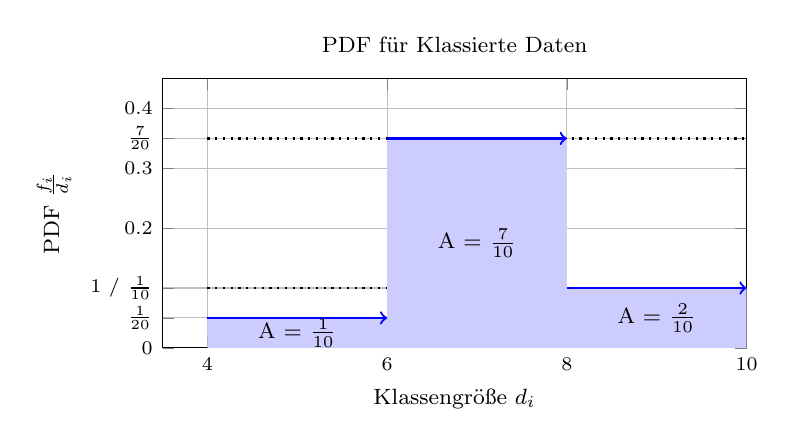
\begin{tikzpicture}
        \begin{axis}
            [
            tick label style={font=\fontsize{7}{7}\selectfont},
            ymin=0, ymax=0.45,
            xmin=3.5, xmax=10,
            xlabel={Klassengröße $d_i$},
            ylabel={PDF $\frac{f_i}{d_i}$},
            xtick={4, 6, 8, 10},
            ytick={0, 0.05, 0.35, 0.1, 0.2, 0.3, 0.4},  % Specify the ytick positions
            yticklabels={0, $\frac{1}{20}$, $\frac{7}{20}$, 1 / $\frac{1}{10}$, 0.2, 0.3, 0.4},  % Override labels with fractions
            title={PDF für Klassierte Daten},
            grid=major,
            width=9cm, height=5cm
            ]

            % Dotted horizontal lines marking the PDF values
            \draw[dotted, thick] (axis cs:4,0.05) -- (axis cs:10,0.05);
            \draw[dotted, thick] (axis cs:4,0.35) -- (axis cs:10,0.35);
            \draw[dotted, thick] (axis cs:4,0.1) -- (axis cs:10,0.1);

            % Fill the area under the PDF plot (without borders)
            \addplot [
                draw=none,
                fill=blue!20, % light blue fill color
                thick,
                domain=4:6
            ] {0.05} \closedcycle;

            \addplot [
                draw=none,
                fill=blue!20, % light blue fill color
                thick,
                domain=6:8
            ] {0.35} \closedcycle;

            \addplot [
                draw=none,
                fill=blue!20, % light blue fill color
                thick,
                domain=8:10
            ] {0.1} \closedcycle;

            % Add the top line as an arrow (and thicker)
            \addplot [
                thick,
                blue,
                -{>[scale=1.5]} % Adds arrow tip at the end
            ] coordinates {
                (4, 0.05) (6, 0.05)
            };

            \addplot [
                thick,
                blue,
                -{>[scale=1.5]} % Adds arrow tip at the end
            ] coordinates {
                (6, 0.35) (8, 0.35)
            };

            \addplot [
                thick,
                blue,
                -{>[scale=1.5]} % Adds arrow tip at the end
            ] coordinates {
                (8, 0.1) (10, 0.1)
            };

            % Add the labels inside the areas
            \node at (axis cs:5, 0.025) {A = $\frac{1}{10}$};
            \node at (axis cs:7, 0.175) {A = $\frac{7}{10}$};
            \node at (axis cs:9, 0.05) {A = $\frac{2}{10}$};

        \end{axis}
    \end{tikzpicture}

% CDF (Cumulative Distribution Function) for Klassierte Data
    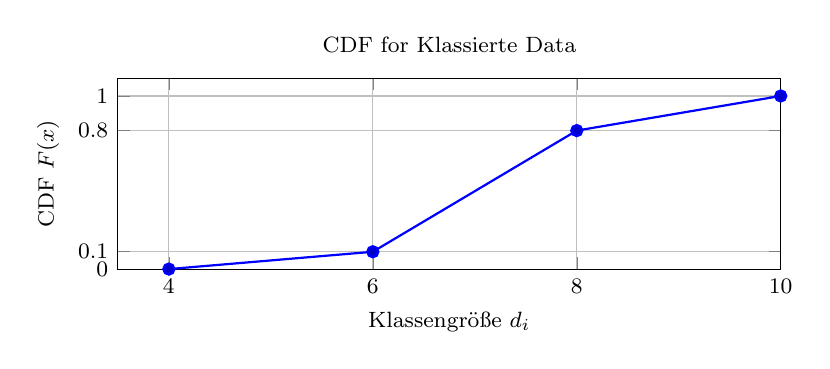
\begin{tikzpicture}
        \begin{axis}
            [
            ymin=0, ymax=1.1,
            xmin=3.5, xmax=10,
            xlabel={Klassengröße $d_i$},
            ylabel={CDF $F(x)$},
            xtick={4, 6, 8, 10},
            ytick={0, 0.1, 0.8, 1},
            title={CDF for Klassierte Data},
            grid=major,
            width=10cm, height=4cm
            ]
            \addplot+[
            const plot,
            sharp plot,
            thick,
            blue
            ] coordinates {
                (4, 0.0)
                (6, 0.1)
                (8, 0.8)
                (10, 1.0)
            };
        \end{axis}
    \end{tikzpicture}

\end{concept}





